
\documentclass[09pt]{article}
\usepackage[margin=1in]{geometry}
\usepackage{graphicx}
\usepackage{enumitem}
\usepackage{listings}
\usepackage{subcaption}
\usepackage{amsthm}
\usepackage{amsmath}
\setlist{nolistsep}
\begin{document}
\lstset{language=Python, numbers=left, tabsize=4}
\begin{center}
\Large{\bf Art Grichine, Adam Beck}\\
\Large{artgrichine@csu.fullerton.edu, adamjbeck@csu.fullerton.edu} \\
\Large{\bf Project 1} 
\end{center}

%=================== Scatter Plots =====================

\vspace{0.2in}
\noindent
\textbf{Scatter Plots:}
\begin{figure}[h]
\centering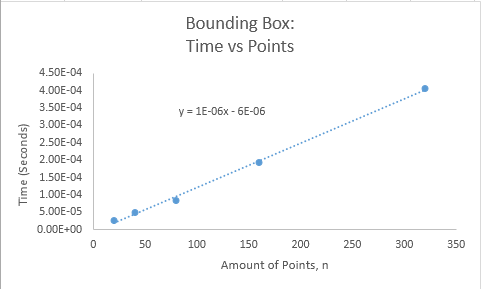
\includegraphics[scale=0.50]{BoundingBoxGraph}
\caption{Bounding Box}
\vspace{0.2in}
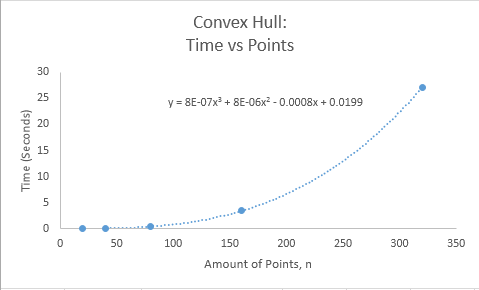
\includegraphics[scale=0.50]{ConvexHullGraph}
\caption{Convex Hull}
\end{figure}

%=================== Pseudocode for both algorithms =====================
%\vspace{2in}
\noindent
\textbf{Pseudocode:} (Bounding Box) \\ \\
The \emph{bounding box} problem is: \\
\indent \textbf{input:} a list of Point objects \\
\indent \textbf{output:} a 4-tuple (x\_min, y\_min, x\_max, y\_max) \\
\begin{lstlisting}[frame=single]
def bounding_box(points):
	initialize x_min, y_min = 1
	initialize x_max, y_max = 0

	for point in points:
		if point.x < x_min:
			x_min = point.x
		if point.x > x_max:
			x_max = point.x
		if point.y < y_min:
			y_min = point.y
		if point.y > y_max:
			y_max = point.y
            
	return x_min, y_min, x_max, y_max
\end{lstlisting}
\vspace{1.25in}
\textbf{Pseudocode:} (Convex Hull) \\ \\
The \emph{convex hull} problem is: \\
\indent \textbf{input:} a list of Point objects \\
\indent \textbf{output:} a list of Point objects on the convex hull boundry\\
\begin{lstlisting}[frame=single]
def convex_hull(points):
	initialize H			#points on the hull boundary
	for point in points:
		for second_point in points:
			if point not equal to second_point
				#find the slope of the line between two points
				m = (second_point.y - point.y)/(second_point.x - point.x)
				
				initialize k = 0
				for third_point in points:
					if not in point or second_point:
						y = m*third_point.x - m*point.x + point.y
						if y less than third_point.y:
							increment k
						
				if k equal 0 or amount of points - 2:
					if point not in H:
						append point to H
					if second_point not in H:
						append second_point to H
	return H	
\end{lstlisting}

%=================== screenshots of n = 20 and n = 200 =====================
\vspace{0.3in}
\noindent
\textbf{Screenshots:} $n = 20$ and $n = 200$\\
\begin{figure}[h]
\centering
\begin{subfigure}[b]{0.45\textwidth}
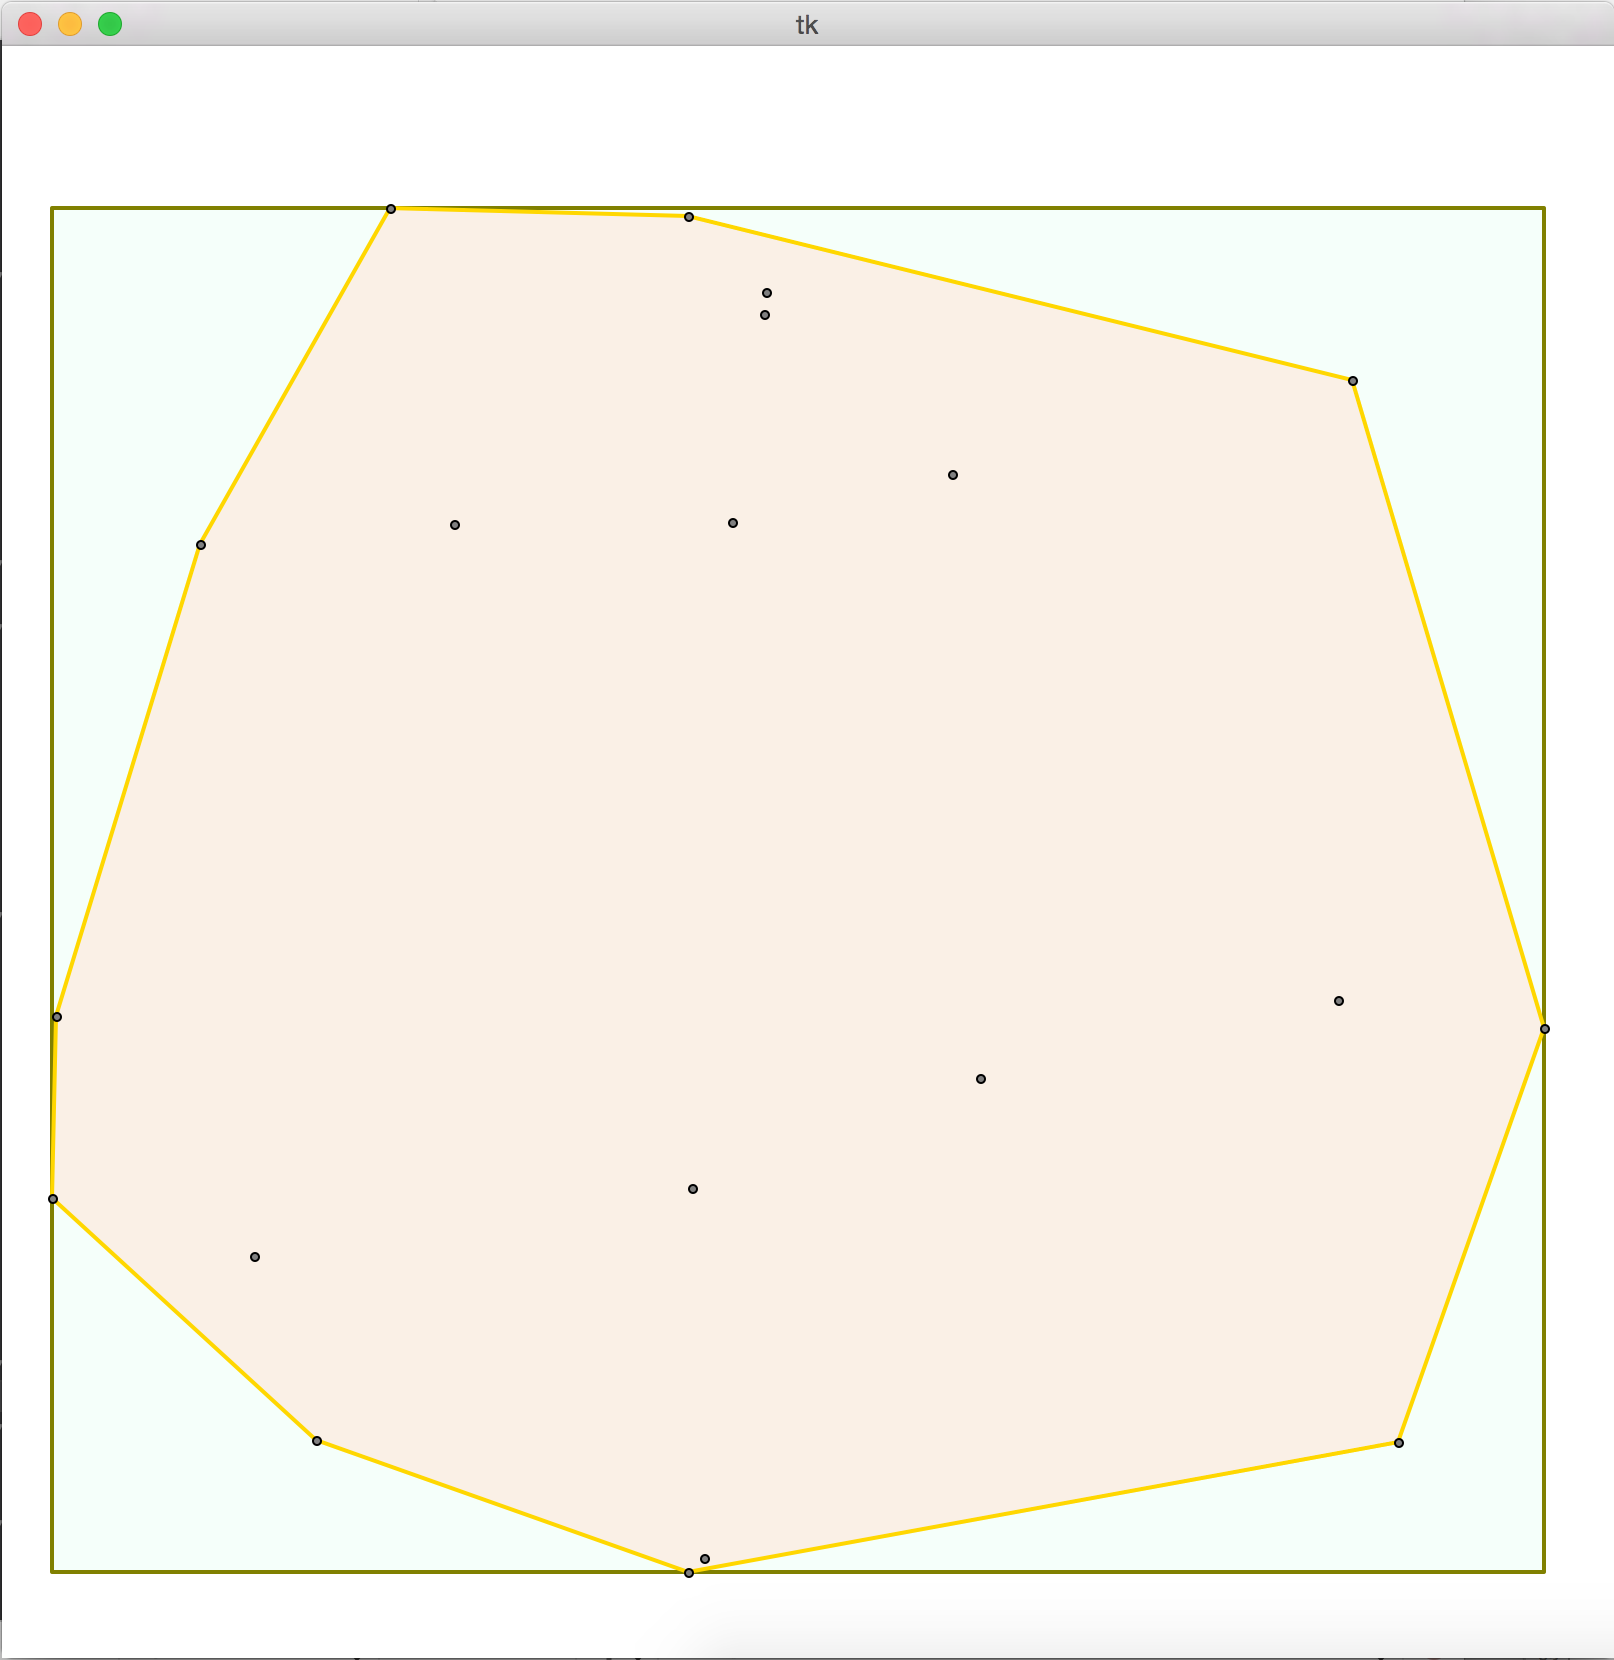
\includegraphics[width=\textwidth]{n_20Points}
\caption{$n = 20$}
\label{fig:1}
\end{subfigure}
\hspace{0.5in}
\begin{subfigure}[b]{0.45\textwidth}
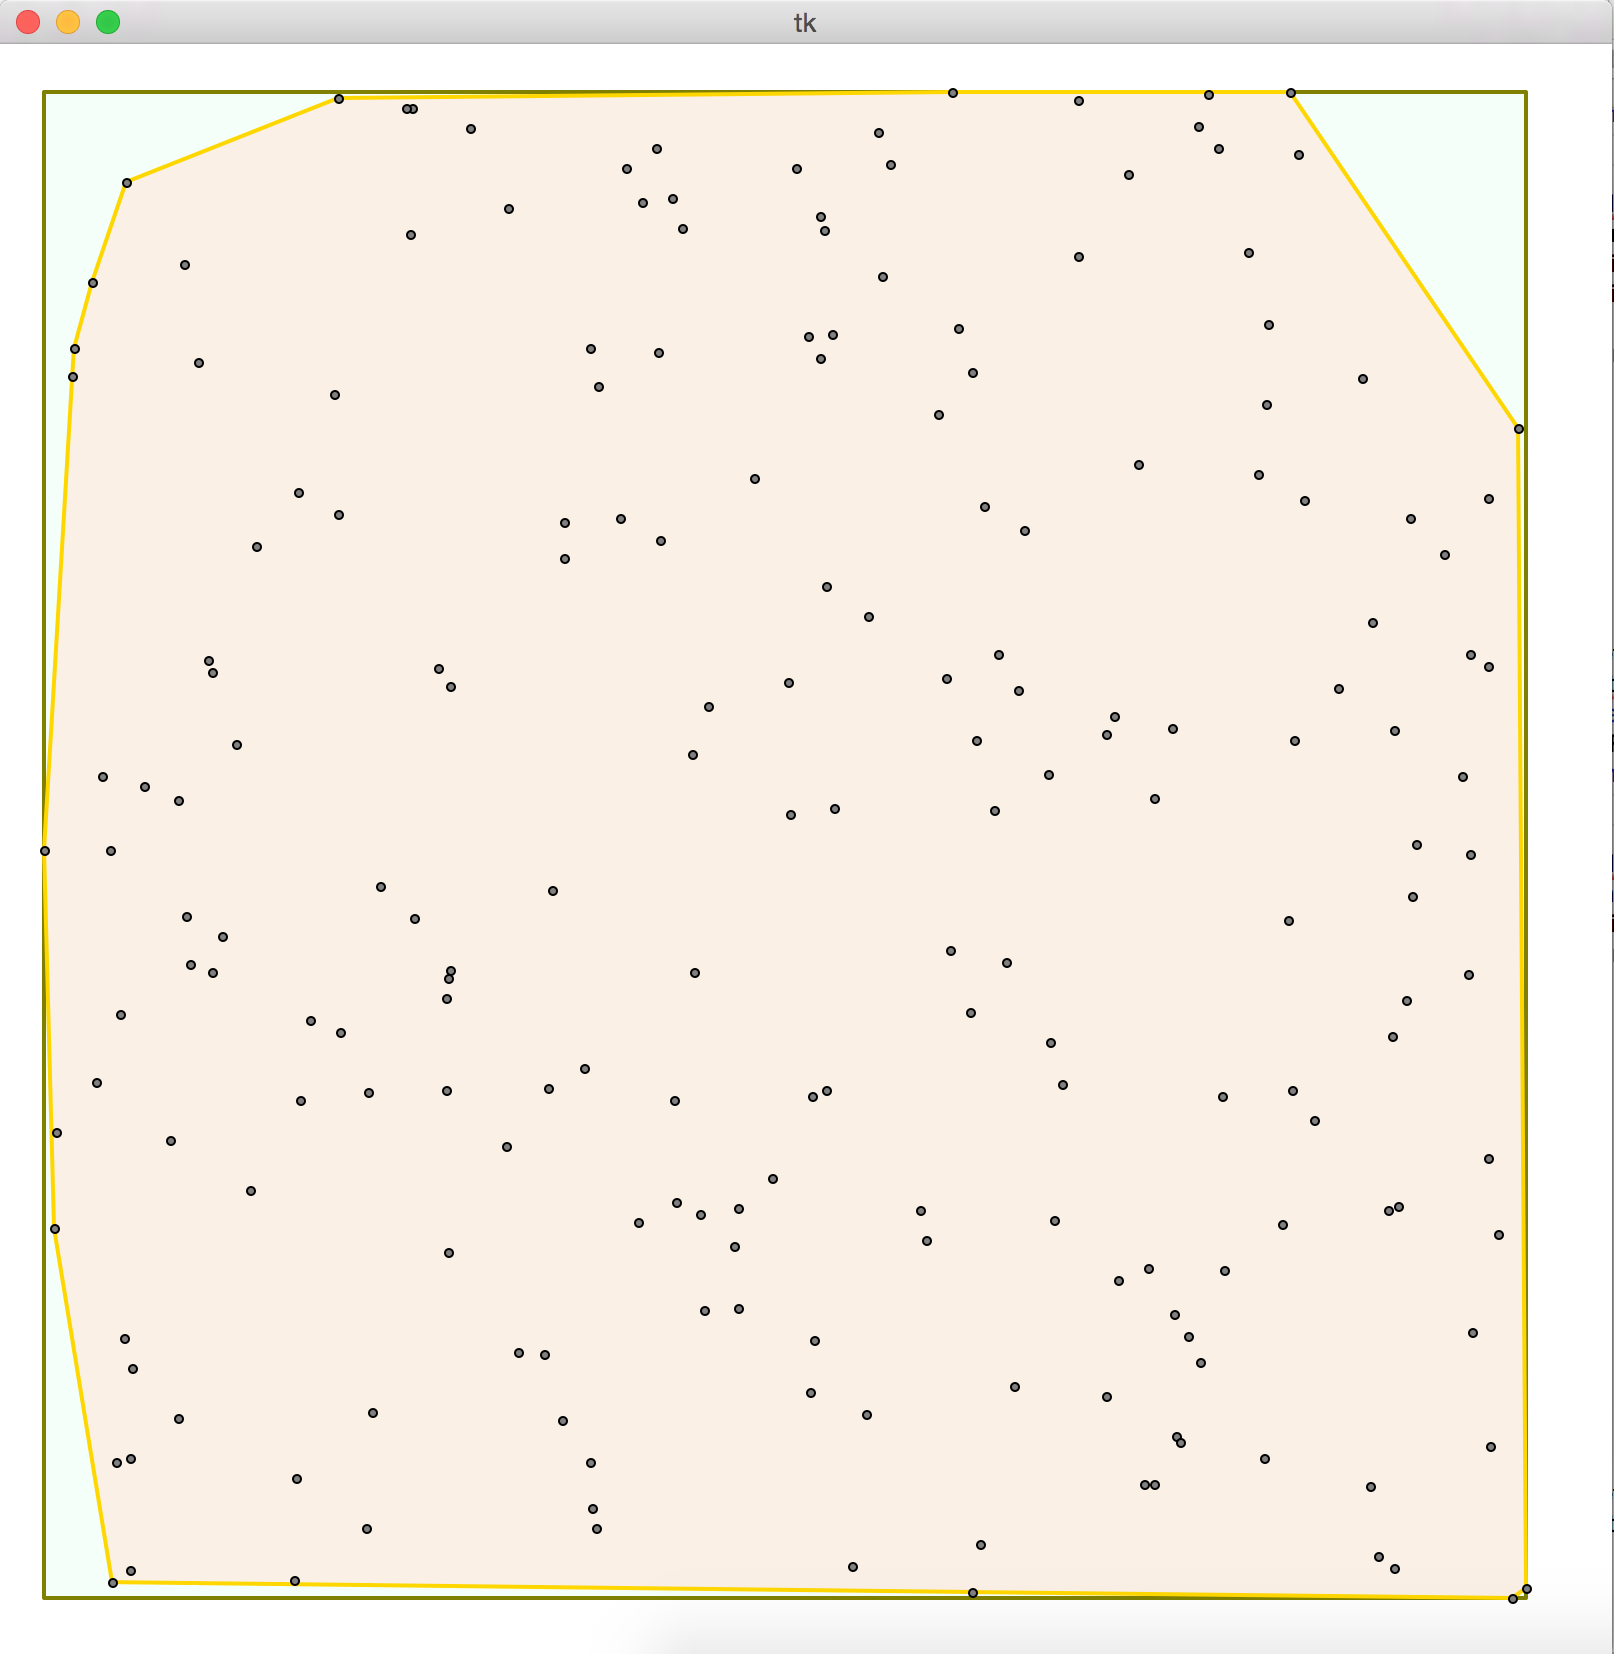
\includegraphics[width=\textwidth]{n_200Points}
\caption{$n = 200$}
\label{fig:2}
\end{subfigure}
\end{figure}

\begin{figure}[h]
\centering
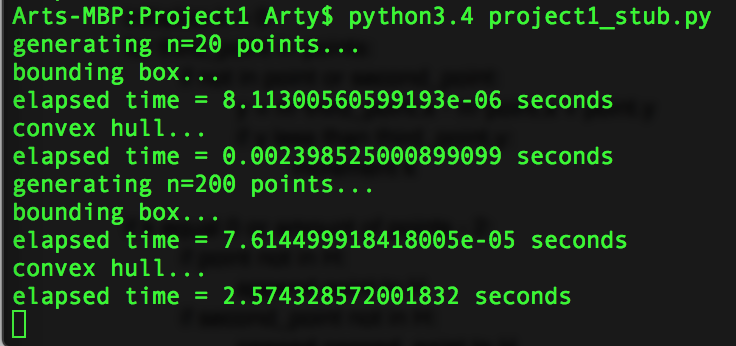
\includegraphics[scale=0.67]{CommandLineOutput}
\caption{Command line output}
\end{figure}

%=================== Questions =====================
\noindent
\textbf{Questions:} \\
\textbf{a.} Is there a noticeable difference in the performance of the two algorithms? Which is faster, and by how much? Does this surprise you? \\

\hangindent=0.2in
Yes; there was a noticeable difference between the two algorithms.  The \emph{bounding box} algorithm is faster by 99.66\% for $n = 20$ and 99.99\% faster for $n=200$.  This result is not surprising, considering the \emph{bounding box} algorithm only uses 1 for-loop. The single for-loop is used to find the points with the minimum and maximum values for $x$ and $y$.  Whereas the \emph{convex hull} algorithm uses 3 for-loops, has to calculate a line between two points, find it's slope, and then compare all other points to the line determining whether or not the line is part of the hull.\\

\noindent
\textbf{b.} What is the efficiency class of each of your algorithms, according to your own mathematical analysis? (You are not required to include all your math work, just state the classes you derived and proved.) \\

\hangindent=0.2in
The derivation for our pseudocode for the \emph{bounding box} problem comes out to be $O(n)$.  The derivation of our pseudocode of the \emph{convex hull} problem comes out to be $O(n^3)$. \\

\noindent
\textbf{c.} Are the fit lines on your scatter plots consistent with these efficiency classes? Justify your answer. \\

\hangindent=0.2in
The best-fit line for our \emph{bounding box} function was very linear, possible errors include machine timing errors. The best-fit line for our \emph{convex hull} graph was cubic, possible errors include machine timing errors. We mathematically derived the time efficiency classes from our pseudocode to be $O(n)$ and $O(n^3)$, then we used the \emph{Excel} software to graph and calculate the best-fit line for our data points.  The best-fit lines came out to be $O(n)$ and $O(n^3)$ for the bounding box and convex hull, respectively, which is consistent with our mathematically derived efficiency classes. \\

\noindent
\textbf{d.} Is this evidence consistent or inconsistent with the hypothesis stated on the first page? Justify your answer. \\

\hangindent=0.2in
Our evidence was consistent with the hypothesis; \\ \\
\emph{``For large values of n, the mathematically-derived efficiency class of an algorithm accurately predicts the observed running time of an implementation of that algorithm"} \\ \\
The observed running times of our graphs came out to be equivalent with the derived efficiency classes.  After using \emph{Excel} to calculate the best-fit line, we compared it to that of our efficiency classes derived from the pseudocode.  Our test data came out to be within the same big-$O$ efficiency class as our derived big-$O$ classes. \\

%=================== Python Code =====================
\vspace{0.2in}
\noindent
\textbf{Python Code:} \\
\begin{lstlisting}[frame=single]
##############################################################################
# CPSC 335 Project 1
# Spring 2015
#
# Authors: Art Grichine, Adam Beck
##############################################################################

# constant parameters
CANVAS_WIDTH = 800
CANVAS_HEIGHT = 800
CANVAS_MARGIN = 20
BOX_OUTLINE_COLOR = 'olive'
BOX_FILL_COLOR = 'mint cream'
HULL_OUTLINE_COLOR = 'gold'
HULL_FILL_COLOR = 'linen'
INTERIOR_POINT_COLOR = 'gray'
POINT_RADIUS = 2
OUTLINE_WIDTH = 2

import math, random, time, tkinter

# Class representing one 2D point.
class Point:
    def __init__(self, x, y):
        self.x = x
        self.y = y

# input: a list of Point objects
# output: a 4-tuple (x_min, y_min, x_max, y_max)
def bounding_box(points):
    #points values range from 0 to 1, we init minimums = 1 and maximums = 0
    x_min, x_max, y_min, y_max = 1,0,1,0        

    for point in points:
        if point.x < x_min:
            x_min = point.x
        if point.x > x_max:
            x_max = point.x
        if point.y < y_min:
            y_min = point.y
        if point.y > y_max:
            y_max = point.y
            
    return(x_min, y_min, x_max, y_max)
    #return (0, 0, 1, 1)            #return this to see entire euclidian plane

# input: a list of Point objects
# output: a list of the Point objects on the convex hull boundary
#Partial code supplied by professor for assignment
def convex_hull(points):
    H = []          #points on the hull boundary
    for point in points:
        for second_point in points:
            if point != second_point:
    #           l = <THE LINE PASSING THROUGH point AND second_point>
    #             equation of line: y-y_1 = m(x - x_1)
    #           calculate slope:
    #             slope = m = (y_2-y_1)/(x_2-x_1)
                m = (second_point.y - point.y)/(second_point.x - point.x)

    #           k = <THE NUMBER OF POINTS ABOVE 1>
    #               With our line's slope calculated, we calculate where the 
    #	            line should be at the third_point's x value. If the 
    #               third_point's y value is greater than the line's y value 
    #               we know that the point is above the line
                k = 0
                for third_point in points:
                    if third_point != point and third_point != second_point:
                        #find the y value for our line
                        y = m*third_point.x - m*point.x + point.y
                        if y < third_point.y:
                            k += 1
    
                if k == 0 or k == len(points)-2:
                    if point not in H:
                        H.append(point)
                    if second_point not in H:
                        H.append(second_point)
    return H

##############################################################################
# The following code is reponsible for generating instances of random
# points and visualizing them. You can leave it unchanged.
##############################################################################

# input: an integer n >= 0
# output: n Point objects with all coordinates in the range [0, 1]
def random_points(n):
    return [Point(random.random(), random.random())
            for i in range(n)]

# translate coordinates in [0, 1] to canvas coordinates
def canvas_x(x):
    return CANVAS_MARGIN + x * (CANVAS_WIDTH - 2*CANVAS_MARGIN)
def canvas_y(y):
    return CANVAS_MARGIN + y * (CANVAS_HEIGHT - 2*CANVAS_MARGIN)

# extract the x-coordinates (or y-coordinates respectively) from a
# list of Point objects
def xs(points):
    return [p.x for p in points]
def ys(points):
    return [p.y for p in points]

# input: a non-empty list of numbers
# output: the mean average of the list
def mean(numbers):
    return sum(numbers) / len(numbers)

# input: list of Point objects
# output: list of the same objects, in clockwise order
def clockwise(points):
    if len(points) <= 2:
        return points
    else:
        center_x = mean(xs(points))
        center_y = mean(ys(points))
        return sorted(points,
                      key=lambda p: math.atan2(p.y - center_y,
                                               p.x - center_x),
                      reverse=True)

# Run one trial of one or both of the algorithms.
#
# 1. Generates an instance of n random points.
# 2. If do_box is True, run the bounding_box algorithm and display its output.
# 3. Likewise if do_hull is True, run the convex_hull algorithm and display
#    its output.
# 4. The run-times of the two algorithms are measured and printed to standard
#    output.
def trial(do_box, do_hull, n):
    print('generating n=' + str(n) + ' points...')
    points = random_points(n)

    if do_box:
        print('bounding box...')
        start = time.perf_counter()
        (x_min, y_min, x_max, y_max) = bounding_box(points)
        end = time.perf_counter()
        print('elapsed time = ' + str(end - start) + ' seconds')

    if do_hull:
        print('convex hull...')
        start = time.perf_counter()
        hull = convex_hull(points)
        end = time.perf_counter()
        print('elapsed time = ' + str(end - start) + ' seconds')

    w = tkinter.Canvas(tkinter.Tk(),
                       width=CANVAS_WIDTH, 
                       height=CANVAS_HEIGHT)
    w.pack()

    if do_box:
        w.create_polygon([canvas_x(x_min), canvas_y(y_min),
                          canvas_x(x_min), canvas_y(y_max),
                          canvas_x(x_max), canvas_y(y_max),
                          canvas_x(x_max), canvas_y(y_min)],
                         outline=BOX_OUTLINE_COLOR,
                         fill=BOX_FILL_COLOR,
                         width=OUTLINE_WIDTH)

    if do_hull:
        vertices = []
        for p in clockwise(hull):
            vertices.append(canvas_x(p.x))
            vertices.append(canvas_y(p.y))

        w.create_polygon(vertices,
                         outline=HULL_OUTLINE_COLOR,
                         fill=HULL_FILL_COLOR,
                         width=OUTLINE_WIDTH)

    for p in points:
        w.create_oval(canvas_x(p.x) - POINT_RADIUS,
                      canvas_y(p.y) - POINT_RADIUS,
                      canvas_x(p.x) + POINT_RADIUS,
                      canvas_y(p.y) + POINT_RADIUS,
                      fill=INTERIOR_POINT_COLOR)

    tkinter.mainloop()

##############################################################################
# This main() function runs multiple trials of the algorithms to
# gather empirical performance evidence. You should rewrite it to
# gather the evidence you need.
##############################################################################
def main():
    n = [20,200]
    for i in n:
        trial(True, True, i)

if __name__ == '__main__':
    main()
\end{lstlisting}


\end{document}